\section{Implementation Details and Practicality}
\label{app:implementation_details}

\begin{table}[t]
\centering
\footnotesize
\setlength{\tabcolsep}{0pt}
\renewcommand{\arraystretch}{1.02}
\begin{tabularx}{\columnwidth}{@{}X@{}}
\toprule
\textbf{Algorithm 1: \sys{} proposal-space inference for image $x$} \\
\midrule
1. Load the frozen prompt-bank proposals $\mathcal{P}(x)$ and compute proposal descriptors $d_i$ for each $m_i \in \mathcal{P}(x)$. \\
2. Score adjacent proposal pairs with $s(i,j)$ and threshold the compatibility graph. \\
3. Form candidate merged regions from the graph connected components. \\
4. Score each candidate with $q(C)$ and choose the conservative core $C^\star = \arg\max_C q(C)$. \\
5. If the route is RWTD, build dense rescue candidates $R_k$ from the auxiliary bank $\mathcal{P}^{+}(x)$. \\
6. Score each $(C^\star, R_k)$ with the safe-switch classifier $p_{\mathrm{safe}}(k)$ and gain regressor $g_{\mathrm{gain}}(k)$. \\
7. Output the positive rescue candidate with highest predicted gain, if any; otherwise output $C^\star$. \\
\bottomrule
\end{tabularx}
\caption{Compact pseudocode for the deployed decision layer. STLD and the appendix routes stop after Step~4 because they do not use the RWTD rescue layer.}
\label{tab:algorithm_box}
\end{table}

\begin{table*}[t]
\centering
\scriptsize
\setlength{\tabcolsep}{4pt}
\renewcommand{\arraystretch}{0.98}
\resizebox{\textwidth}{!}{%
\begin{tabular}{@{}llcccccc@{}}
\toprule
Benchmark / subset & Output & \multicolumn{2}{c}{Handcrafted-only} & \multicolumn{2}{c}{PTD-only} & \multicolumn{2}{c}{Hybrid} \\
 &  & mIoU & ARI & mIoU & ARI & mIoU & ARI \\
\midrule
RWTD common-253 & Stage-A official & 0.4469 & 0.6556 & 0.4486 & 0.6505 & 0.4558 & 0.6812 \\
RWTD full-256 & Stage-A official & 0.4454 & 0.6533 & 0.4472 & 0.6484 & 0.4543 & 0.6786 \\
STLD common-182 & Stage-A direct & 0.7045 & 0.7808 & 0.6698 & 0.7740 & 0.7195 & 0.7791 \\
STLD all-200 & Stage-A direct & 0.6570 & 0.7265 & 0.6253 & 0.7203 & 0.6705 & 0.7249 \\
\bottomrule
\end{tabular}
}
\caption{Descriptor ablation for the descriptor-sensitive Stage-A commitment layer, with the proposal bank, evaluator, and model family held fixed. RWTD is reported at Stage-A because the dense rescue layer operates on candidate masks and is unchanged across descriptor variants. Hybrid descriptors are clearly strongest on RWTD, while STLD is less sensitive to the descriptor choice and even slightly favors handcrafted-only on ARI.}
\label{tab:descriptor_ablation}
\end{table*}

\begin{table*}[t]
\centering
\scriptsize
\setlength{\tabcolsep}{3pt}
\renewcommand{\arraystretch}{0.98}
\begin{tabularx}{\textwidth}{@{}p{0.14\textwidth}ccccccX@{}}
\toprule
Route & Prompt props & Merged comps & Dense props & Rescue cand. & s / img & Peak RSS & Reading \\
\midrule
RWTD Stage-A & 3.84 & 2.64 & -- & -- & 0.025 & 430 MiB & prompt-bank commitment only \\
RWTD full & 3.84 & 2.64 & 38.05 & 11.72 & 0.378 & 637 MiB & dense rescue evaluated on the full set; 21/256 images switch \\
STLD Stage-A & 1.78 & 2.32 & -- & -- & -- & -- & no rescue path; no separate runtime profile recorded \\
\bottomrule
\end{tabularx}
\caption{Practicality profile of the deployed decision layer. RWTD timings come from measured full-dataset GPU profiles of the same frozen-bank pipeline. STLD shares the same Stage-A architecture and bank statistics, but no separate runtime profile was recorded in the repository.}
\label{tab:practicality}
\end{table*}


\paragraph{Why include this appendix section?} The paper's main claim is scientific rather than systems-oriented, but two reviewer questions still matter: whether the gain depends mainly on a particular descriptor stack, and whether the decision layer is practical enough to deploy above a frozen bank. The tables in this section answer those questions directly. The descriptor ablation keeps the decision stack fixed while varying only the proposal descriptor in the descriptor-sensitive Stage-A layer; on RWTD, hybrid descriptors help clearly more than either single family, while STLD is noticeably less sensitive and sometimes slightly favors handcrafted cues on ARI. The practicality table then summarizes the actual bank sizes, rescue scale, and measured runtime profile of the deployed RWTD and STLD routes.

\section{Feature-Space Evidence}
\label{app:feature_provenance}

The feature-space route is reported under its archived probe protocol. Its repository-backed artifacts come from the coarse-feature clustering bundles, the parity summaries, and the scale-probe study in the \texttt{research-site} tree. The key caveat is short and fixed throughout this appendix: the RWTD feature probe does not use the official proposal-route evaluator, so this route is read as evidence for where texture structure can already live inside frozen features rather than merged into the matched proposal-route tables.

\begin{figure*}[t]
    \centering
    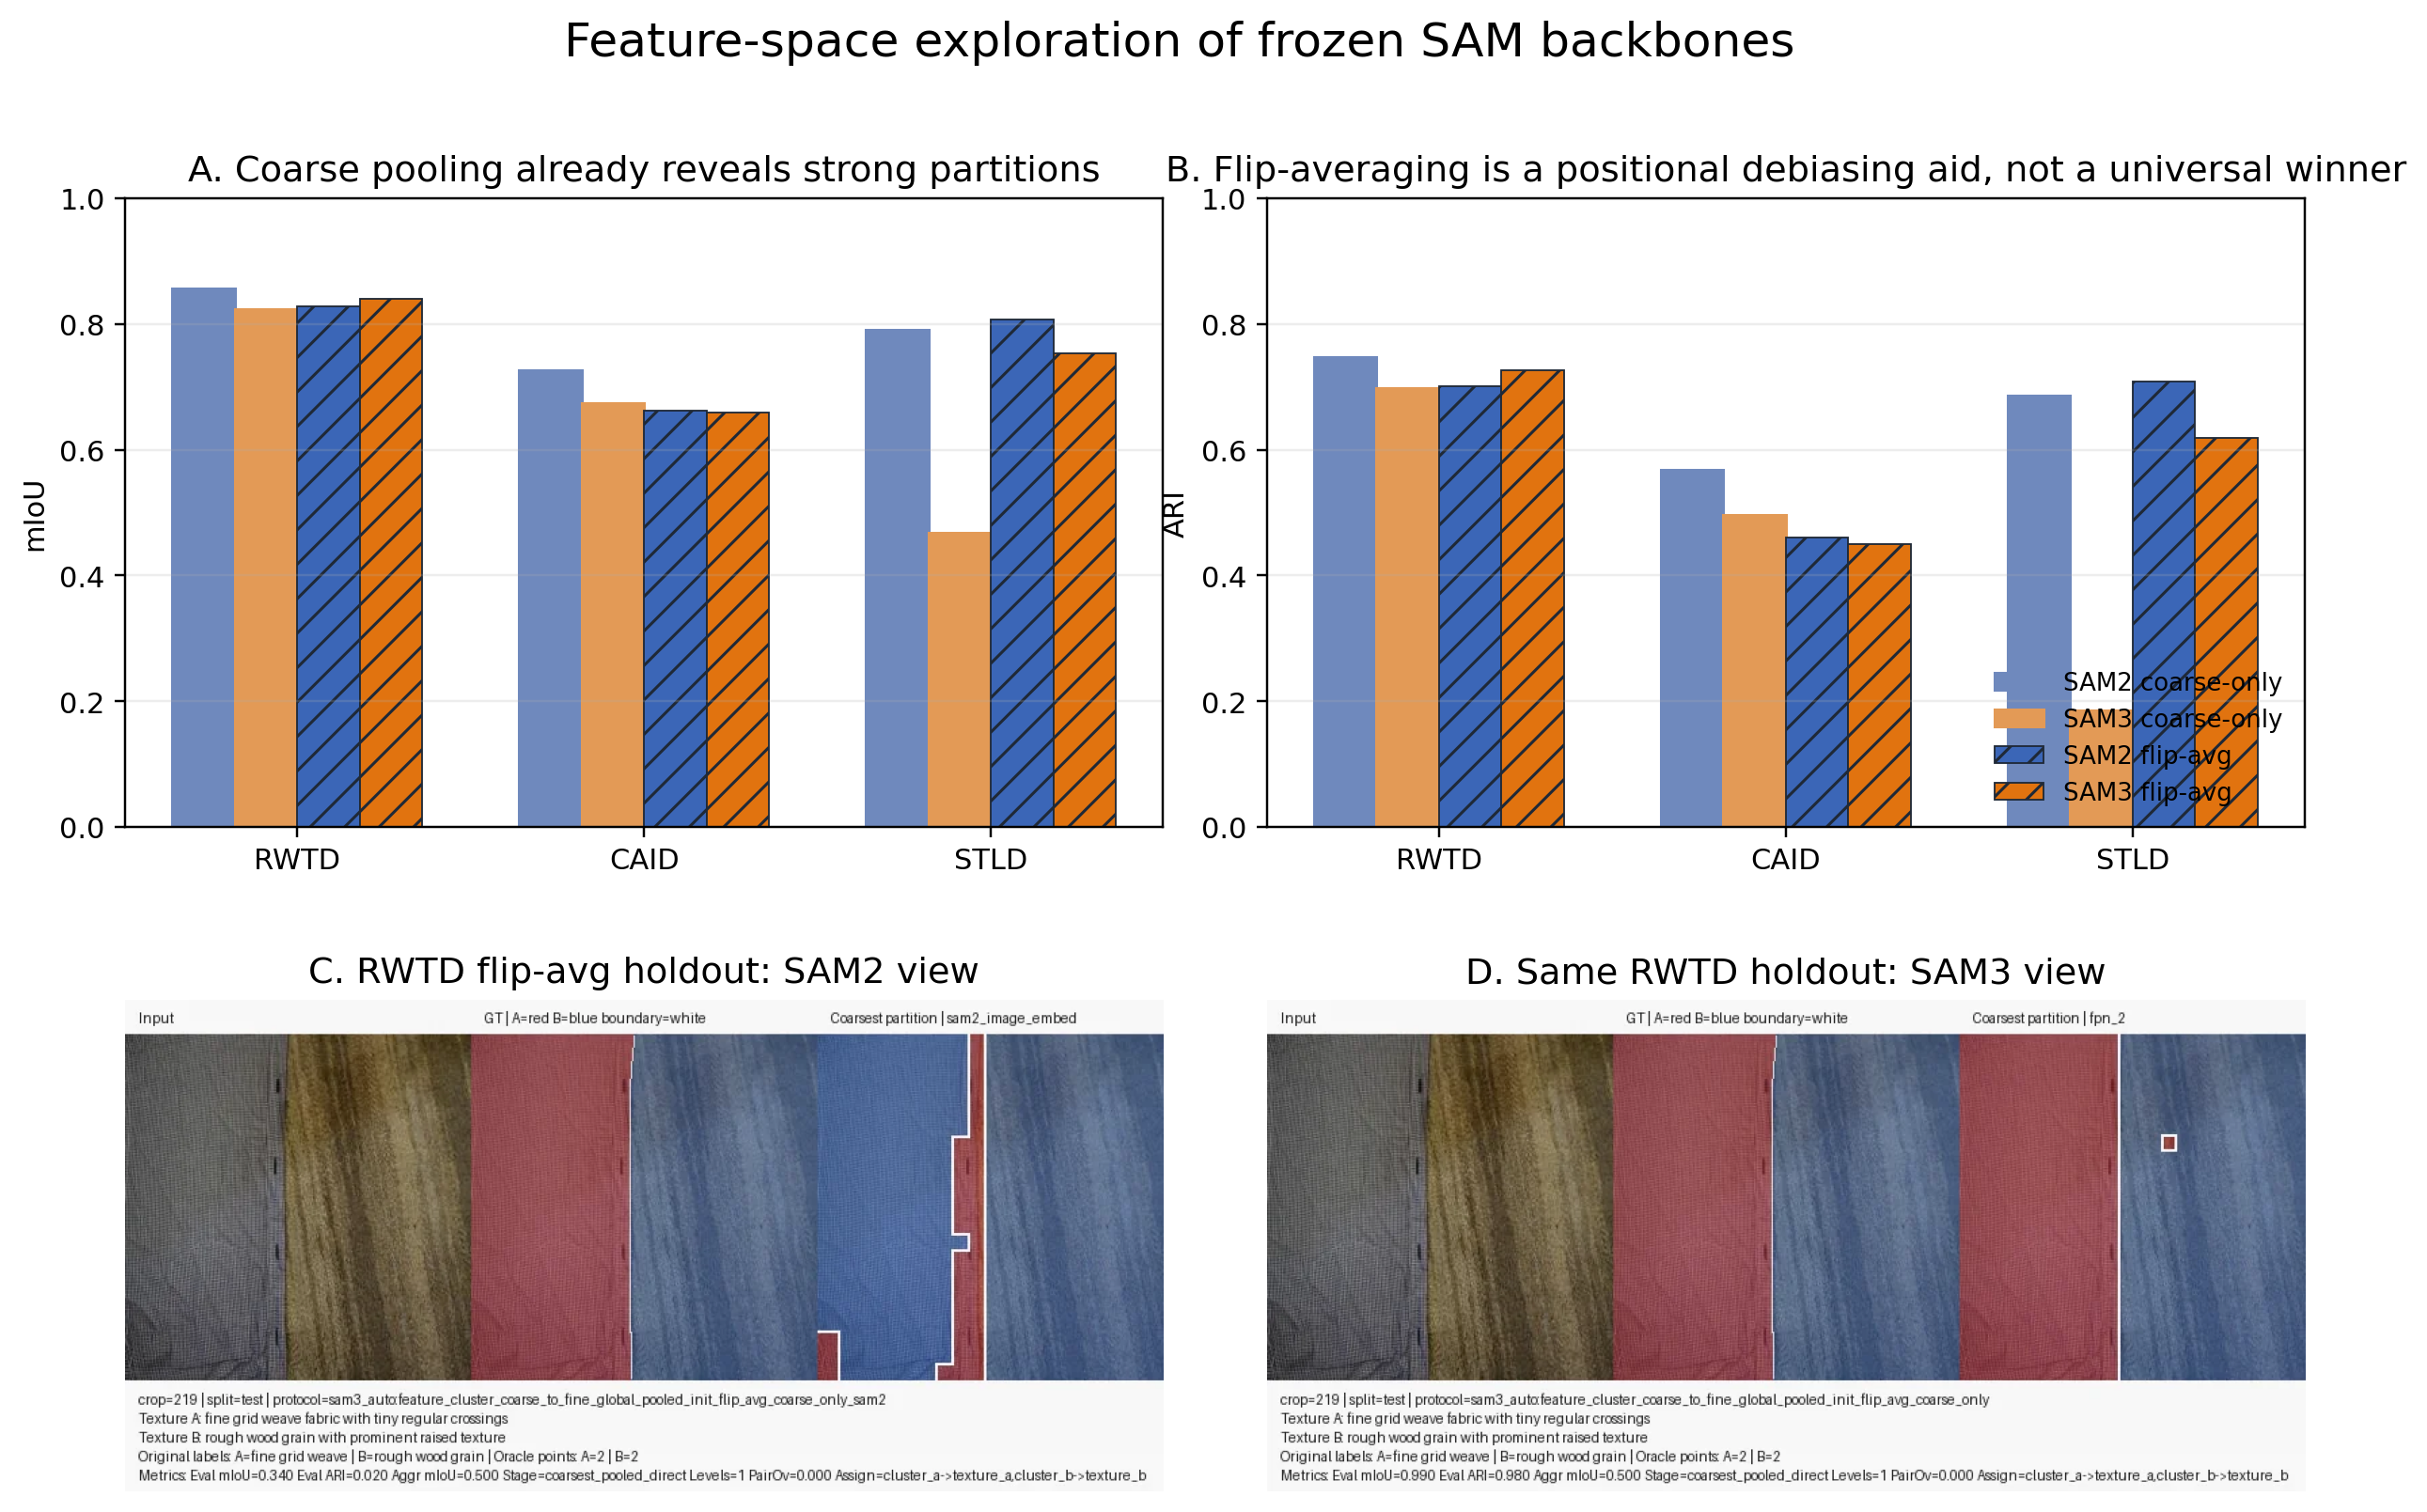
\includegraphics[width=0.98\textwidth]{figures/fig_feature_space_recovery.png}
    \caption{Archived feature-probe summary from the repository parity bundles. Top: coarse-only and flip-averaged summaries across RWTD, STLD, and CAID. Bottom: representative RWTD holdouts showing that coarse clustering can recover plausible binary partitions while remaining sensitive to positional bias.}
    \label{fig:feature_summary_app}
\end{figure*}

\begin{figure*}[t]
    \centering
    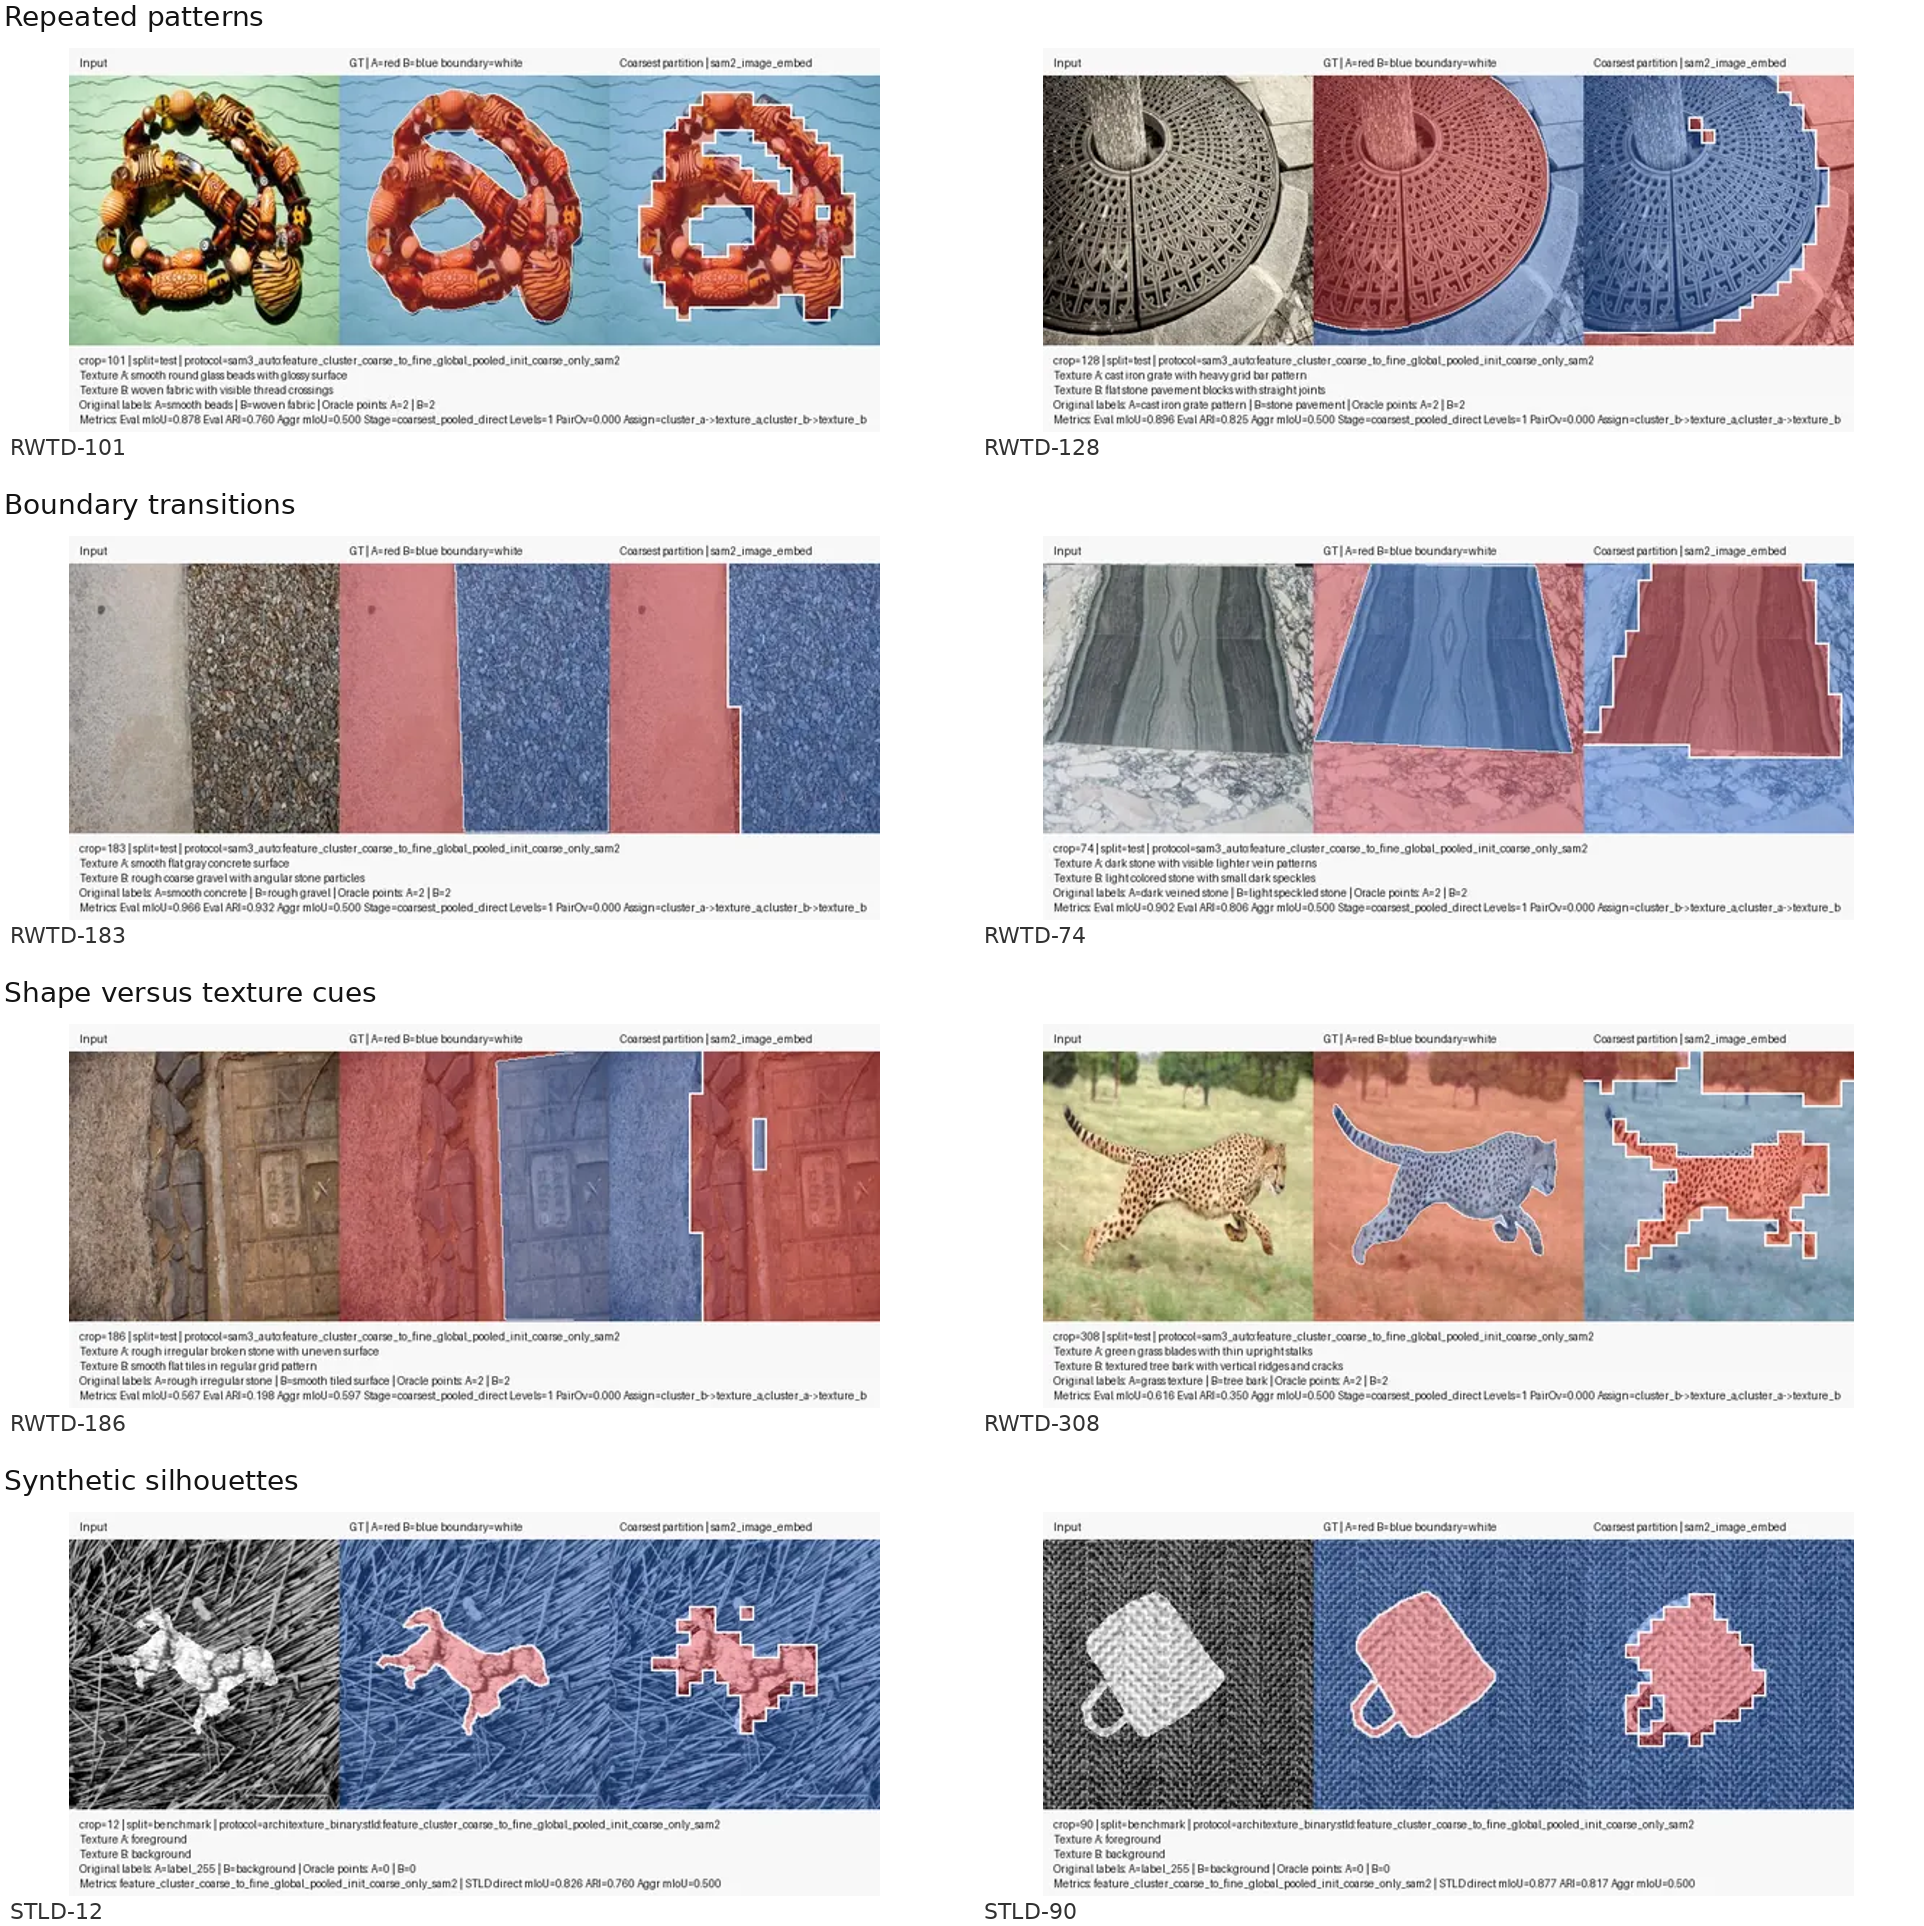
\includegraphics[width=0.98\textwidth]{figures/fig_feature_gallery.png}
    \caption{Curated qualitative gallery for coarse frozen-feature clustering. The gallery spans repeated-pattern scenes, gradual texture transitions, shape-versus-texture cases, and synthetic silhouettes. The annulus example in RWTD-101 is representative of the strongest qualitative evidence: even a frozen coarse probe can recover a topologically nontrivial partition without retraining the backbone.}
    \label{fig:feature_gallery}
\end{figure*}

\begin{figure*}[t]
    \centering
    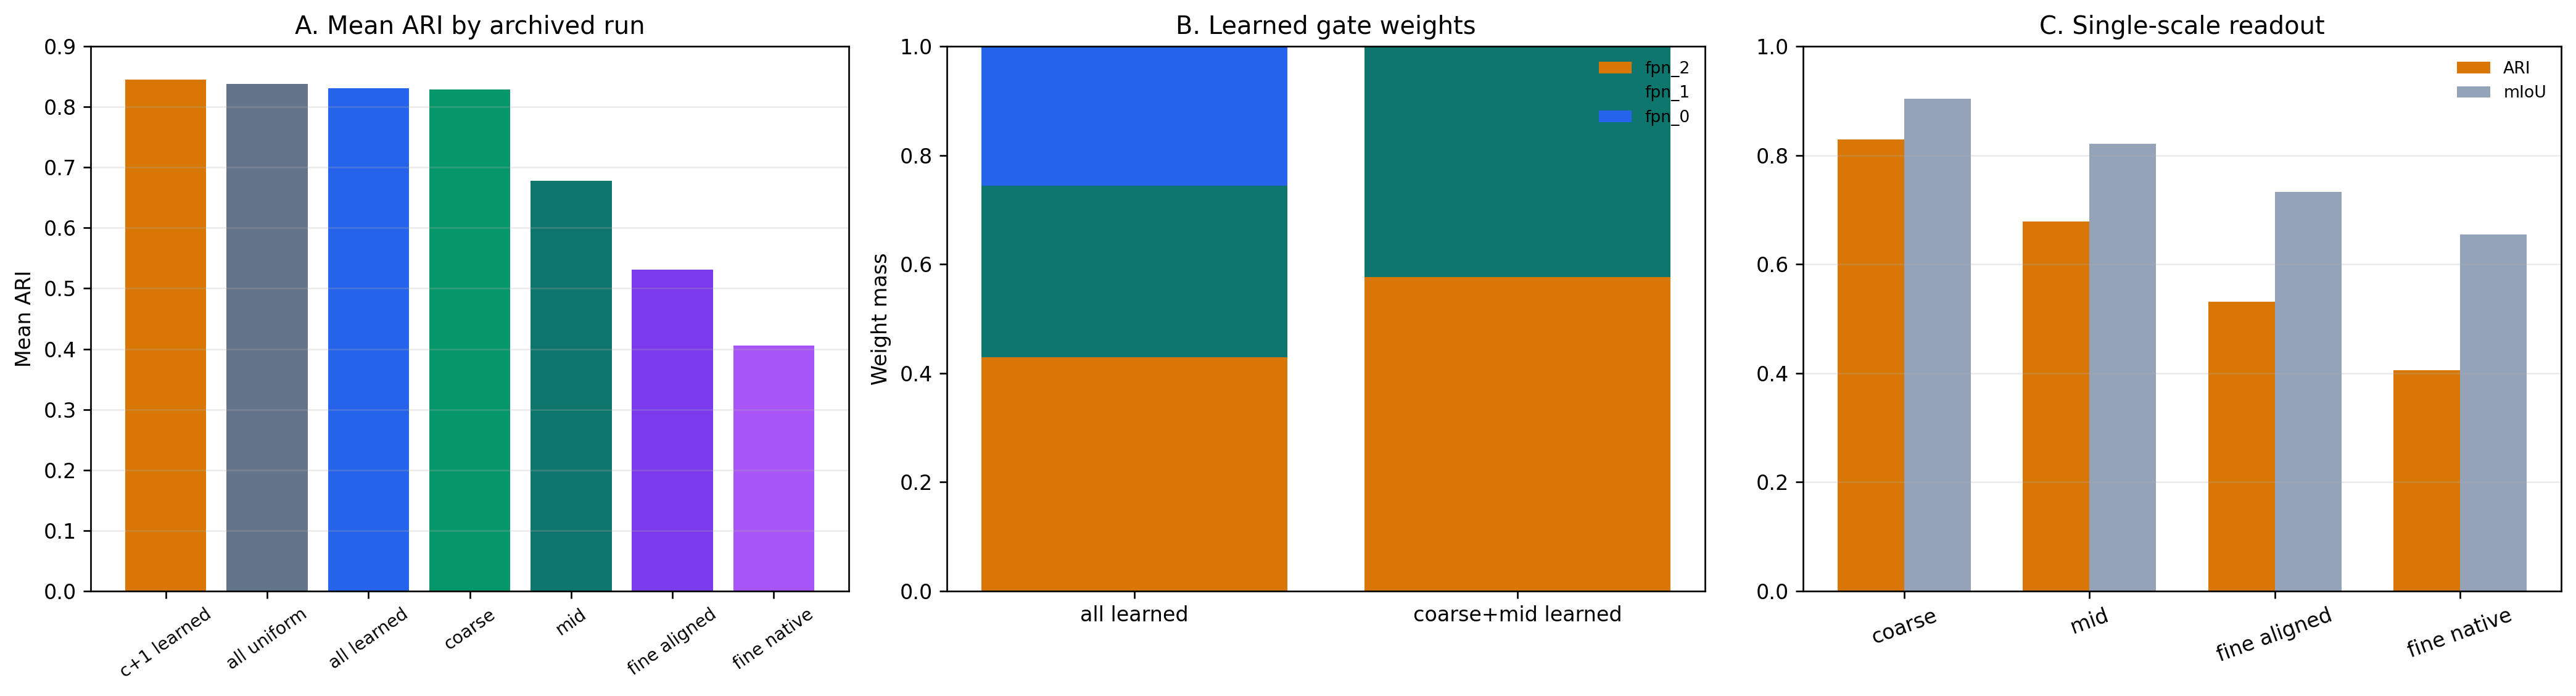
\includegraphics[width=0.98\textwidth]{figures/fig_feature_scale_diagnostics.png}
    \caption{Archived scale and gating diagnostics from the feature probe. Left: mean ARI by run. Middle: learned all-scale and coarse-plus-mid gate weights still place most mass on the coarsest level. Right: single-scale readouts show that coarse features dominate, while native fine-grid clustering is the weakest control. These runs are read as archived probe evidence rather than as matched benchmark comparisons.}
    \label{fig:feature_scale_diag}
\end{figure*}

\paragraph{Interpretation.} The appendix diagnostics point in one direction. Coarse frozen features already recover much of the binary partition on the repository-backed probe, learned all-scale fusion still prefers the coarsest level, and the finest native grid is the least reliable setting. That is enough for the paper's use of this route: frozen SAM features can contain texture-aware structure, even though the feature probe is not the matched benchmark route used for RWTD and STLD headline comparisons.

\begin{table}[t]
\centering
\scriptsize
\setlength{\tabcolsep}{4pt}
\renewcommand{\arraystretch}{0.98}
\resizebox{\columnwidth}{!}{%
\begin{tabular}{@{}llcccc@{}}
\toprule
Dataset & Eval view & SAM2 coarse-only & SAM3 coarse-only & SAM2 flip-avg & SAM3 flip-avg \\
\midrule
RWTD & partition-invariant & 0.8561 / 0.7472 & 0.8235 / 0.6984 & 0.8278 / 0.7013 & 0.8397 / 0.7258 \\
CAID & partition-invariant & 0.7263 / 0.5673 & 0.6743 / 0.4956 & 0.6620 / 0.4605 & 0.6588 / 0.4507 \\
STLD & direct foreground & 0.7908 / 0.6864 & 0.4682 / 0.1859 & 0.8064 / 0.7089 & 0.7534 / 0.6194 \\
\bottomrule
\end{tabular}
}
\caption{Archived frozen-feature parity summary from the site bundle. Each cell is reported as mIoU / ARI. This table is reported under the archived feature-probe protocol and is not merged into the matched proposal-route benchmark tables.}
\label{tab:feature_parity}
\end{table}


\section{RWTD Oracle and Failure Details}
\label{app:rwtd_diag}

RWTD is where the recoverability claim is most demanding. The proposal bank is strong, but the deployed decision stack still leaves a large oracle gap. \Cref{fig:rwtd_case_gallery} shows four recurring patterns. First, top-1 proposal scoring can miss cases where conservative component commitment succeeds. Second, rescue can repair an under-covered core. Third, a strong singleton can already exist in the bank even when the deployed stack abstains from it. Fourth, the remaining wrong-partition failures are low-margin commitment mistakes rather than proposal-bank misses.

\begin{figure*}[t]
    \centering
    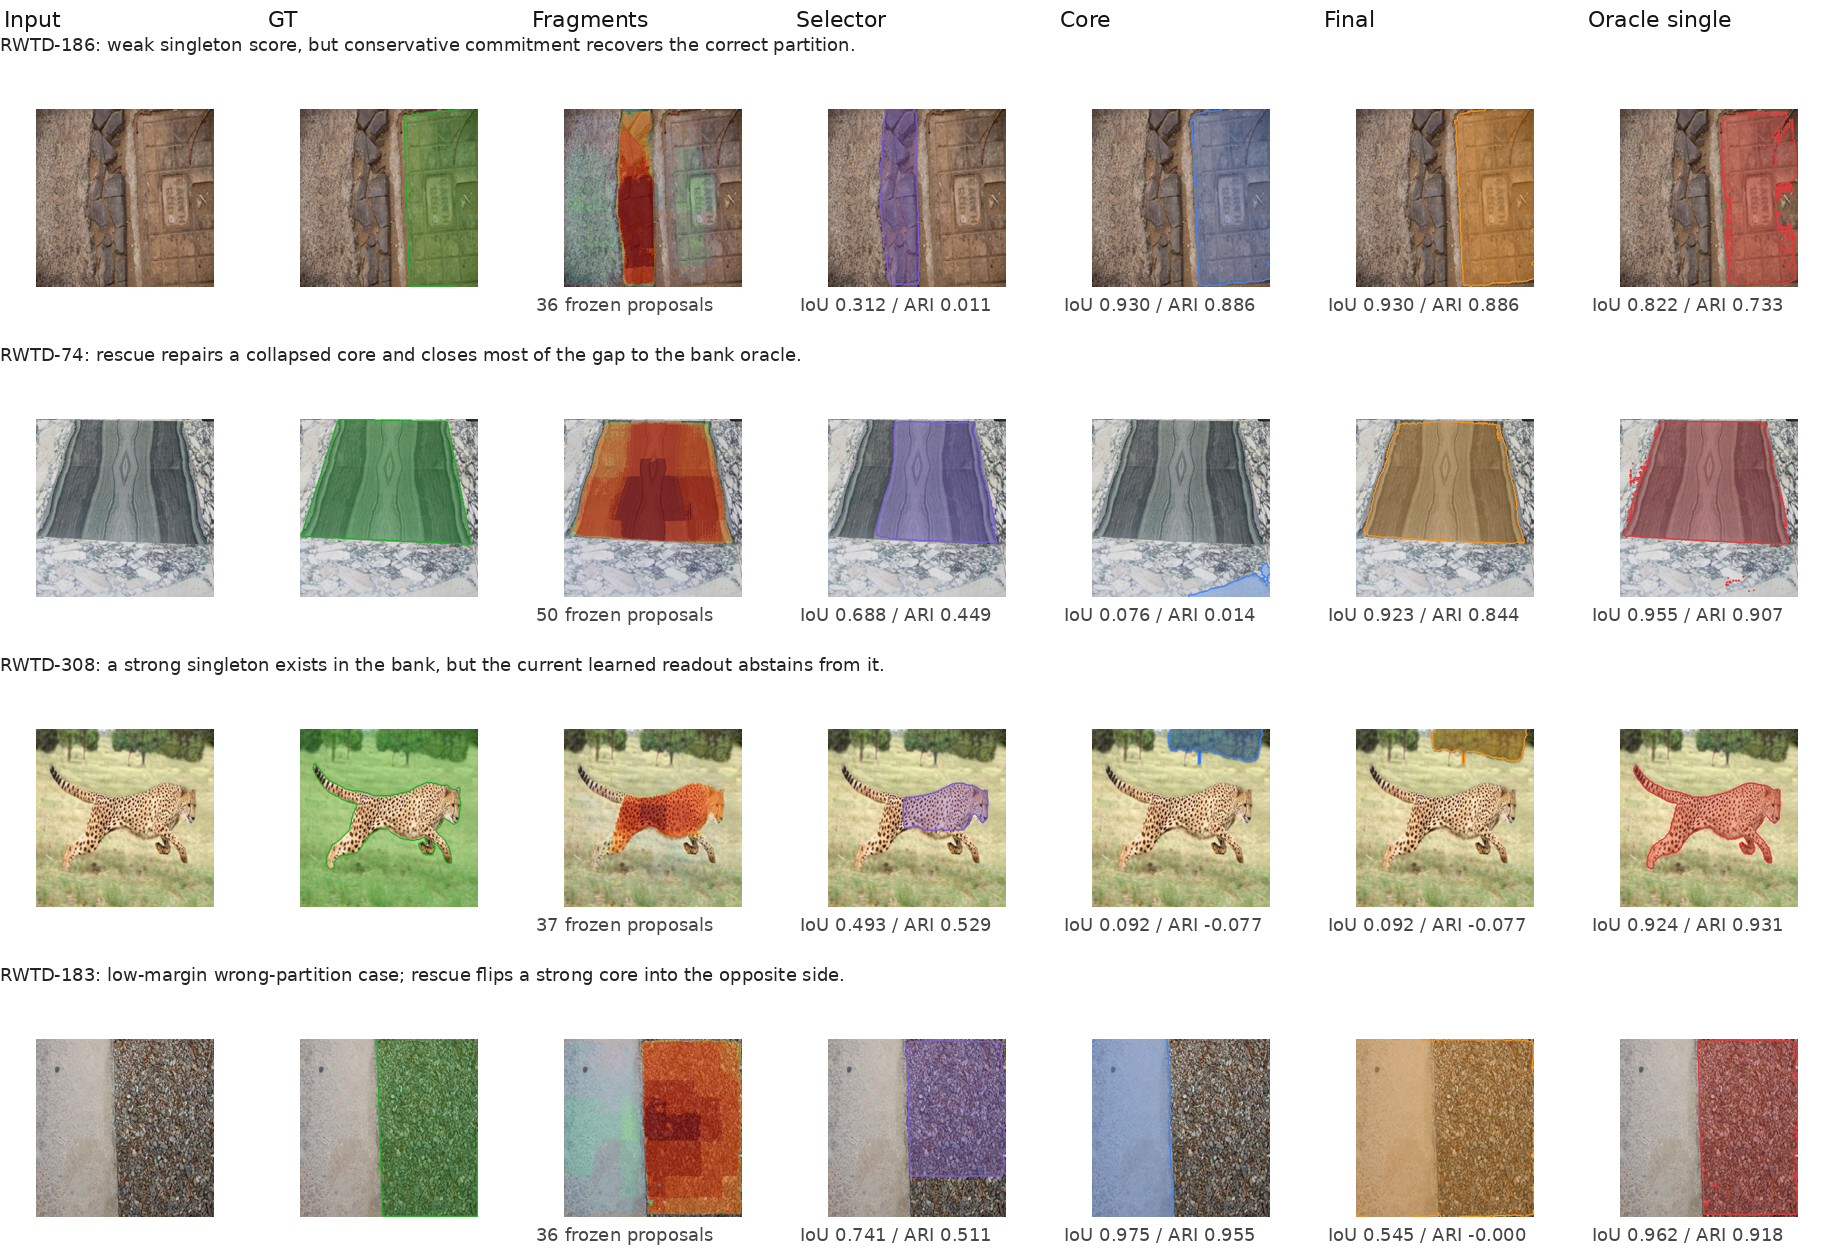
\includegraphics[width=\textwidth]{figures/fig_rwtd_case_gallery.png}
    \caption{RWTD case studies across selector, core, final, and oracle views. These examples make the oracle gap concrete: the bank often contains a strong answer, but the deployed stack still needs the right commitment decision to reach it. The rescue layer helps on some under-coverage cases, but low-margin wrong-partition failures remain brittle.}
    \label{fig:rwtd_case_gallery}
\end{figure*}

\begin{figure*}[t]
    \centering
    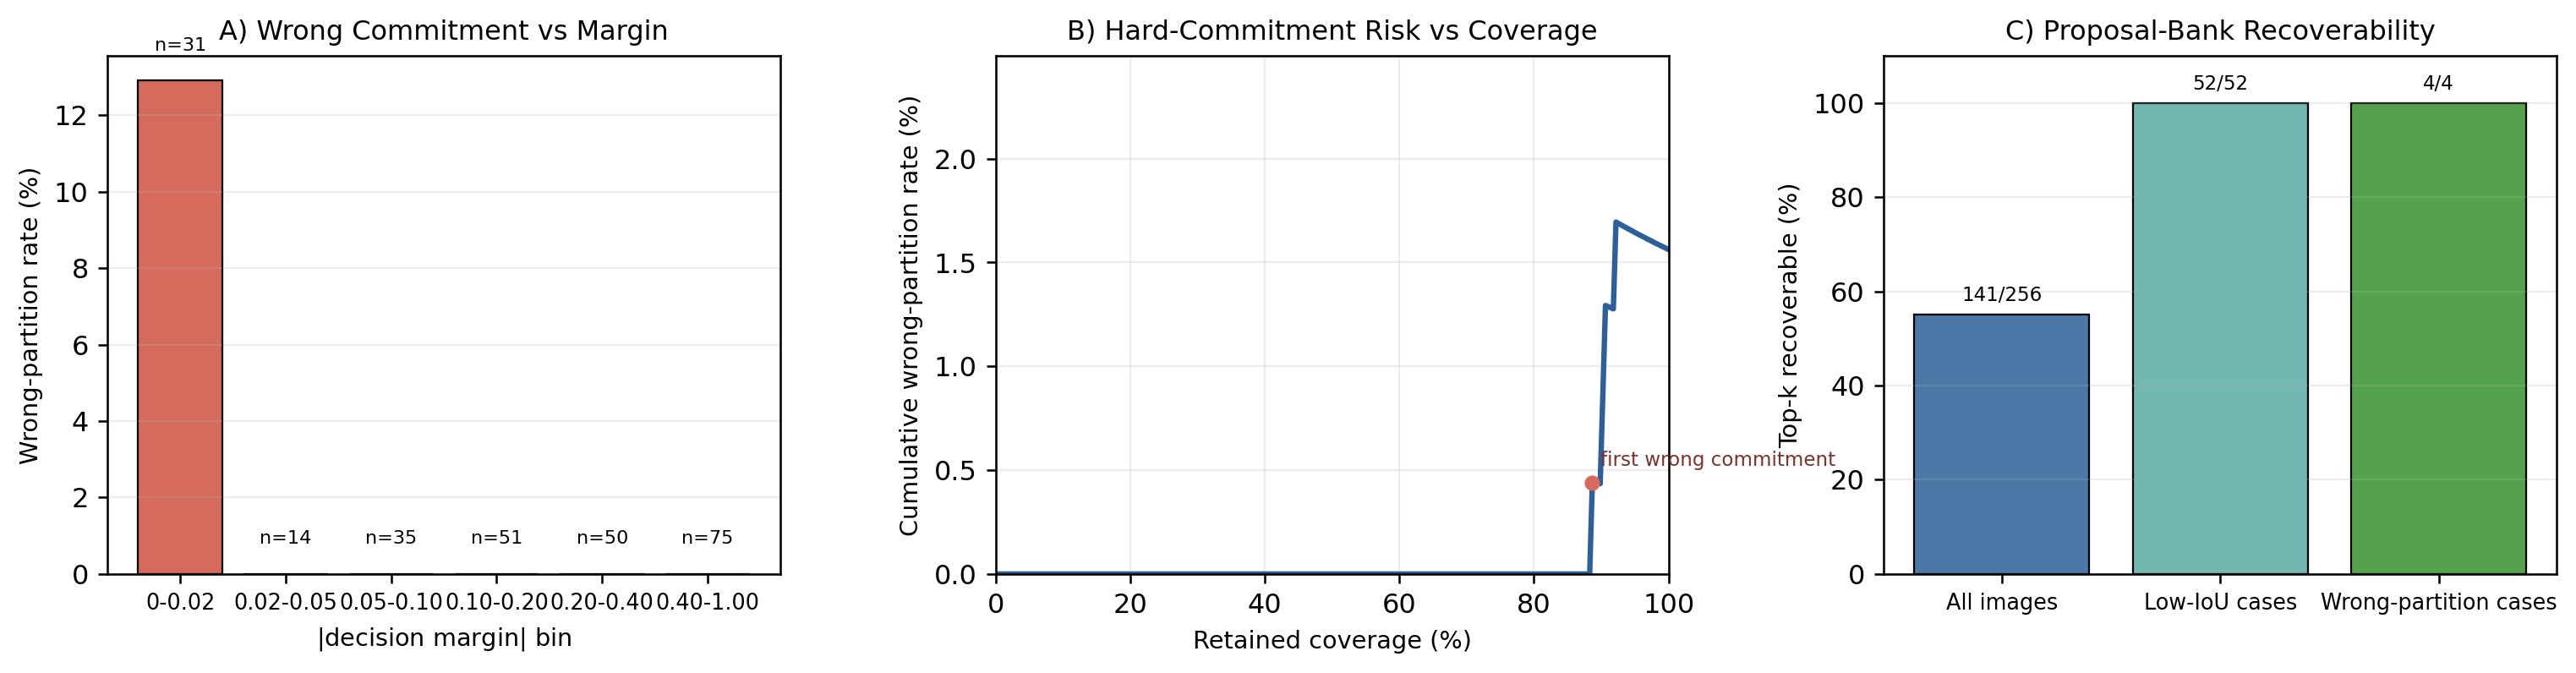
\includegraphics[width=0.92\textwidth]{figures/fig_ambiguity_commitment_full256.png}
    \caption{RWTD ambiguity-to-failure diagnostics on the full-256 audit. Wrong-partition cases concentrate in the lowest-margin regime, and top-$k$ recoverability remains high exactly where the final decision layer is most brittle.}
    \label{fig:ambiguity_commitment}
\end{figure*}

\paragraph{How to read the oracle gap.} The bank upper bound is not a deployable method: it assumes access to the ground-truth partition when choosing among proposals, merged components, and rescue candidates. Its role is diagnostic. On RWTD, the gap between the deployed system and that bound shows that the frozen bank already contains more usable texture evidence than the current decision layer recovers. The learned single-selector baseline narrows only part of that gap, which is why RWTD still needs structured commitment above fragmented proposals.

\begin{table*}[t]
\centering
\small
\begin{tabularx}{\textwidth}{@{}Xccccccc@{}}
\toprule
Setting & Resc. & Off-succ. & Hurt-any & Wrong & Unsafe & Mean $\Delta$IoU & Top-$k$ recov. \\
\midrule
Baseline decision rule & 21 & 61.9\% & 38.1\% & 4 & 6 & +0.2247 & 141/256 \\
\bottomrule
\end{tabularx}
\caption{RWTD full-256 failure-audit summary for the deployed decision rule. The remaining weakness is ambiguity-aware commitment rather than proposal-bank absence.}
\label{tab:rwtd_audit}
\end{table*}

\begin{table*}[t]
\centering
\scriptsize
\begin{tabularx}{\textwidth}{@{}Xcc@{}}
\toprule
Dense rescue proposal source (frozen) & Full-256 mIoU / ARI & Common-253 mIoU / ARI \\
\midrule
Released dense bank & 0.4611 / 0.6966 & 0.4645 / 0.7013 \\
SAM2.1-large source swap & 0.5003 / 0.7048 & 0.5005 / 0.7106 \\
\bottomrule
\end{tabularx}
\caption{Frozen proposal-source transfer stress test. Consolidation weights and thresholds remain fixed; only the rescue proposal bank changes. This is evidence for modularity of the decision layer, not a standalone benchmark claim.}
\label{tab:proposal_swap}
\end{table*}

\begin{table*}[t]
\centering
\scriptsize
\setlength{\tabcolsep}{5pt}
\renewcommand{\arraystretch}{0.98}
\begin{tabularx}{\textwidth}{@{}p{0.22\textwidth}p{0.17\textwidth}cc@{}}
\toprule
Comparison & Paired units & $\Delta$ mIoU (95\% interval) & $\Delta$ ARI (95\% interval) \\
\midrule
RWTD common-253, \sys{} $-$ TextureSAM & 426 overlapped GT instances & $+0.0405$ [$0.0031$, $0.0764$] & $+0.0995$ [$0.0721$, $0.1270$] \\
STLD all-200, \sys{} $-$ TextureSAM & 200 images & $+0.2028$ [$0.1555$, $0.2486$] & $+0.0400$ [$0.0049$, $0.0754$] \\
STLD common-182, \sys{} $-$ TextureSAM & 182 images & $+0.2055$ [$0.1558$, $0.2518$] & $+0.0265$ [$-0.0097$, $0.0605$] \\
\bottomrule
\end{tabularx}
\caption{Paired interval support for the matched comparisons. RWTD uses the official overlap-instance view because the published no-aggregation metric averages GT instances overlapped by each method rather than simple per-image means. STLD intervals are paired per-image bootstraps under the direct-foreground evaluator.}
\label{tab:bootstrap_support}
\end{table*}

\begin{table*}[t]
\centering
\small
\begin{tabularx}{\textwidth}{@{}p{0.30\textwidth}X@{}}
\toprule
Item & Value \\
\midrule
External training data & PTD only for RWTD, the ADE20K-selected complement, the ControlNet bridge complement, and the appendix CAID route; Brodatz-native synthetic supervision for STLD \\
Encoder training data & 80{,}000 train / 20{,}000 val images per synthetic source \\
RWTD benchmark usage & Evaluation only; no RWTD-label training or hyperparameter search \\
Proposal source & Frozen SAM-style automatic masks \\
RWTD / STLD deployed model & Swin-Base masked-region encoder with learned merge/core/repair modules \\
ADE20K / ControlNet / CAID appendix deployed model & PTD-trained \texttt{small\_pre\_ring\_hi} Stage-A bundle \\
Primary evaluator & Official upstream no-aggregation evaluator on RWTD; route-matched evaluators elsewhere \\
Comparator family & Raw SAM2.1-small plus reproduced/public TextureSAM checkpoints \\
\bottomrule
\end{tabularx}
\caption{Compact reproducibility summary for the manuscript scope.}
\label{tab:compact_repro}
\end{table*}


\section{STLD Supporting Oracle Analysis}
\label{app:stld_support}

STLD plays a different supporting role. The oracle analysis still shows extra headroom in the bank, but the learned top-1 selector is already close to the full system on the common-182 subset. In practice, many STLD images contain a coherent singleton answer, so the main remaining gain is modest coherence cleanup rather than large-scale fragment commitment.

\begin{table*}[t]
\centering
\scriptsize
\begin{tabularx}{\textwidth}{@{}XccccX@{}}
\toprule
Dataset / subset & Selector mIoU & Selector ARI & Final mIoU & Final ARI & Reading \\
\midrule
RWTD common-253 & 0.4512 & 0.5601 & 0.4645 & 0.7013 & Large ARI gap: fragmented natural scenes still need structured commitment above the frozen bank. \\
STLD common-182 & 0.7196 & 0.7731 & 0.7195 & 0.7791 & Near-parity: a coherent singleton answer often already exists, so commitment adds only a small coherence gain. \\
\bottomrule
\end{tabularx}
\caption{Cross-dataset contrast between learned top-1 selection and full proposal-space commitment. RWTD and STLD use different evaluators, so the point is not absolute scale but the different role played by singleton selection on the two routes.}
\label{tab:stld_selector_contrast}
\end{table*}


\begin{figure*}[t]
    \centering
    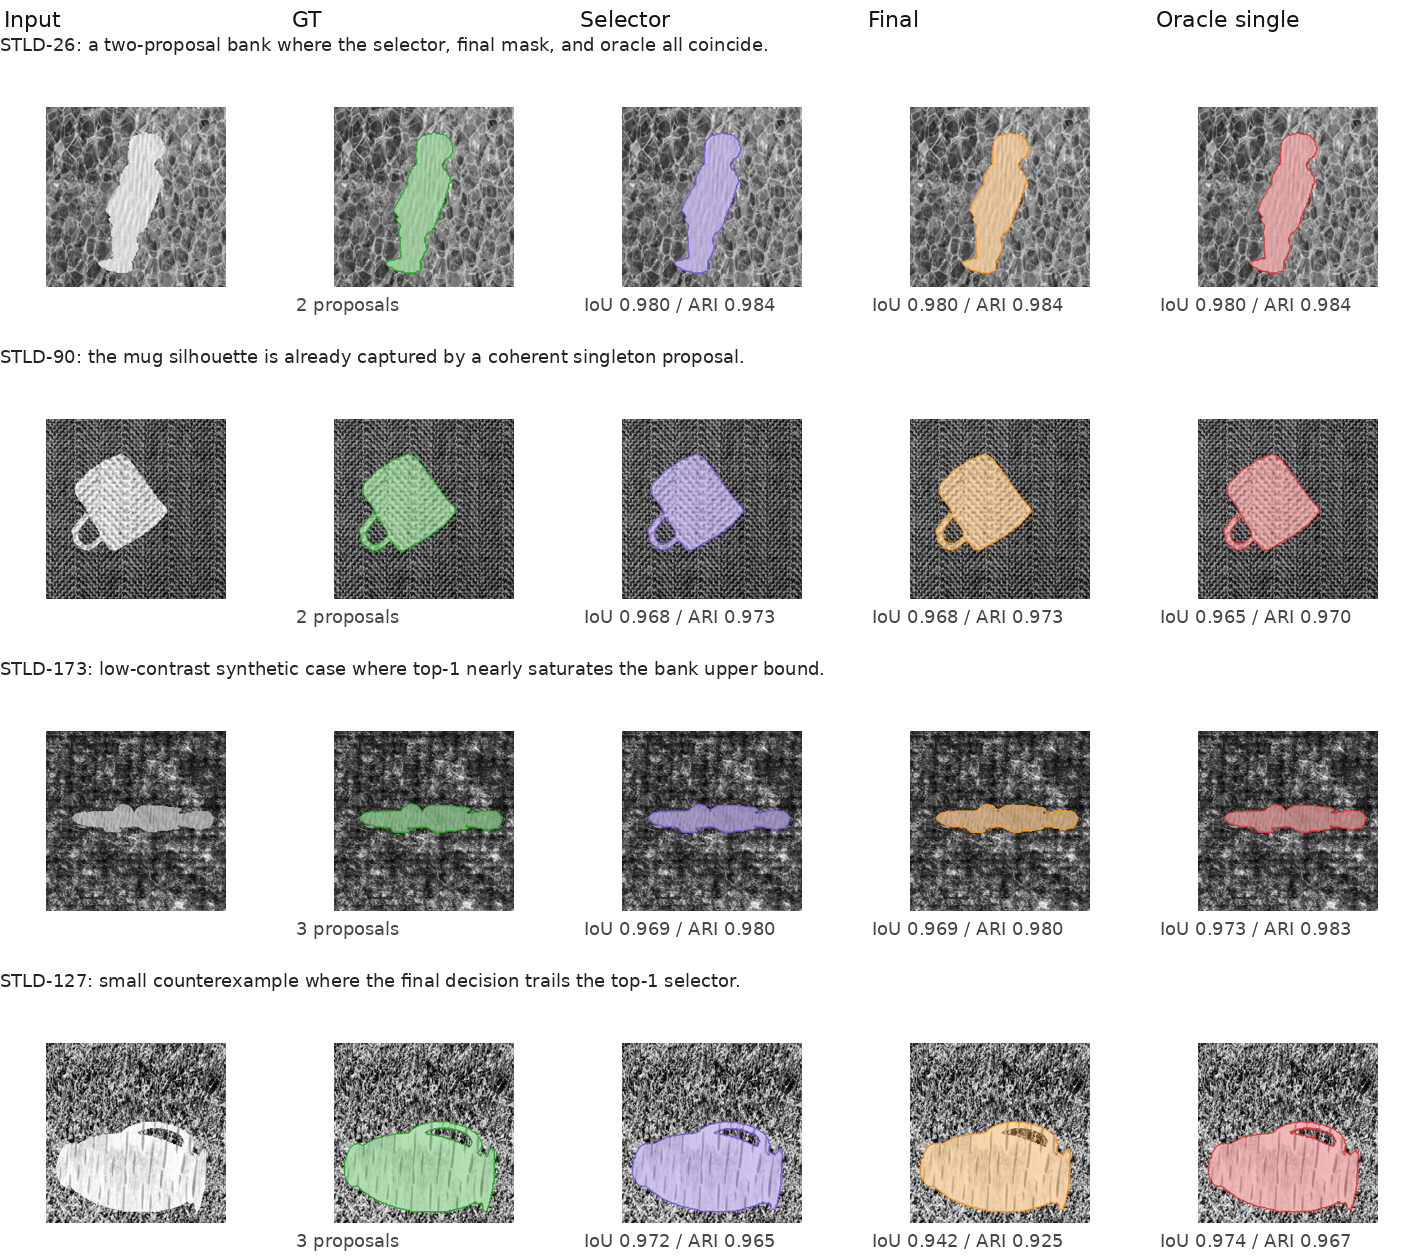
\includegraphics[width=0.96\textwidth]{figures/fig_stld_case_gallery.png}
    \caption{Representative STLD cases. Most examples already have a coherent singleton proposal, so the learned selector, final deployment, and single-proposal oracle are nearly indistinguishable. The last row shows a useful counterexample where the selector slightly outruns the final decision.}
    \label{fig:stld_case_gallery}
\end{figure*}

\begin{table*}[t]
\centering
\scriptsize
\setlength{\tabcolsep}{5pt}
\renewcommand{\arraystretch}{0.98}
\begin{tabular}{@{}lcccc@{}}
\toprule
STLD method & All-200 mIoU & All-200 ARI & Common-182 mIoU & Common-182 ARI \\
\midrule
Proposal route final & 0.6705 & 0.7249 & 0.7195 & 0.7791 \\
Learned single selector & 0.6548 & 0.7036 & 0.7196 & 0.7731 \\
Single frozen-proposal oracle & 0.7375 & 0.7684 & 0.8105 & 0.8444 \\
Compatible-component oracle & 0.3950 & 0.3598 & 0.4341 & 0.3953 \\
Top-$k$ union oracle & 0.1257 & 0.0289 & 0.1381 & 0.0317 \\
Bank upper bound & 0.7574 & 0.7962 & 0.8149 & 0.8574 \\
\bottomrule
\end{tabular}
\caption{Supporting STLD oracle analysis under the direct-foreground evaluator. The learned top-1 selector already recovers much of the overlap on STLD, but the full proposal-route readout remains slightly stronger on coherence and still trails the bank oracles.}
\label{tab:stld_oracles}
\end{table*}


\section{Supporting Routes}
\label{app:route_secondary}

The remaining routes stay secondary by design. The ControlNet-stitched bridge benchmark preserves exact supervision while introducing more naturalistic transitions than hard mosaics, but this paper does not claim a causal bridge-training benefit. CAID is kept only as a breadth check under domain shift.

\subsection{ControlNet Bridge Examples}
\label{app:bridge_secondary}

\begin{figure*}[t]
    \centering
    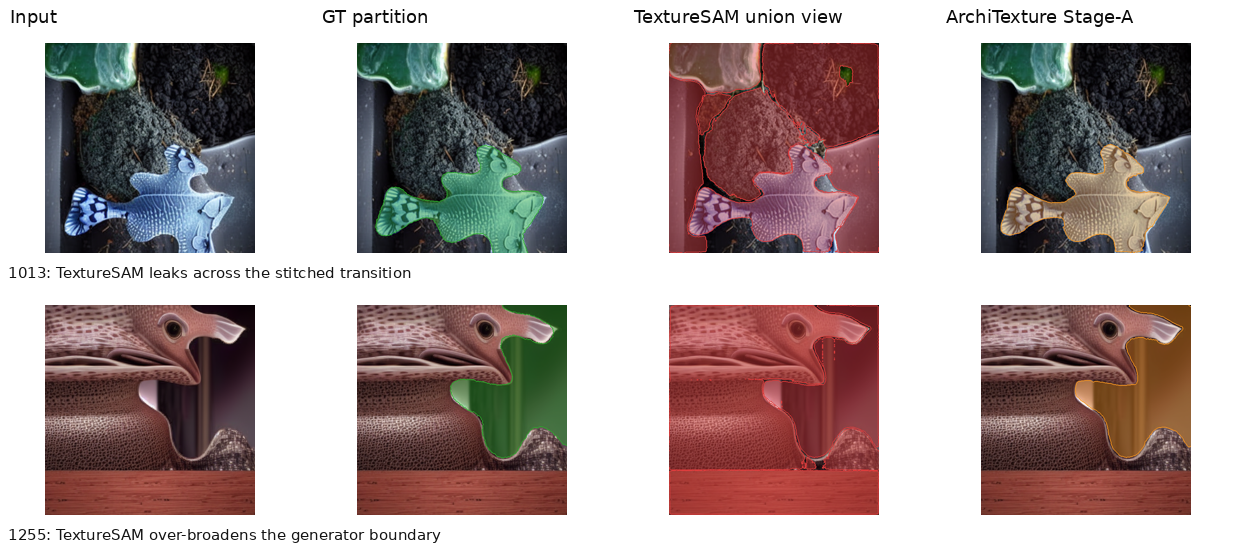
\includegraphics[width=0.92\textwidth]{figures/fig_controlnet_bridge_examples.png}
    \caption{ControlNet-stitched bridge examples. The proposal-union view often leaks across the stitched transition or over-broadens the generator boundary, which explains why overlap can look reasonable while ARI remains fragile. The Stage-A route is more conservative, but we keep this benchmark in the appendix because the paper does not establish a causal bridge-training advantage.}
    \label{fig:controlnet_bridge_app}
\end{figure*}

\begin{table*}[t]
\centering
\scriptsize
\begin{tabularx}{\textwidth}{@{}Xlcc@{}}
\toprule
Method & Subset / coverage & Direct mIoU / ARI & Invariant mIoU / ARI \\
\midrule
TextureSAM public checkpoint rerun & all-1742, 1739/1742 & 0.4212 / 0.6446 & 0.6425 / 0.5510 \\
Proposal route Stage-A & all-1742, 1742/1742 & 0.4993 / 0.6039 & 0.6803 / 0.6039 \\
TextureSAM public checkpoint rerun & common-1739 & 0.4219 / 0.6457 & 0.6436 / 0.5519 \\
Proposal route Stage-A & common-1739 & 0.4993 / 0.6039 & 0.6803 / 0.6039 \\
\bottomrule
\end{tabularx}
\caption{ControlNet-stitched synthetic complement. This route broadens the synthetic side beyond the classical STLD benchmark by preserving exact labels while using more naturalistic stitched transitions. The main text emphasizes the invariant view; this appendix table retains the direct and matched-subset views together.}
\label{tab:controlnet_secondary}
\end{table*}


\subsection{CAID Breadth Check}
\label{app:caid_secondary}

\begin{figure*}[t]
    \centering
    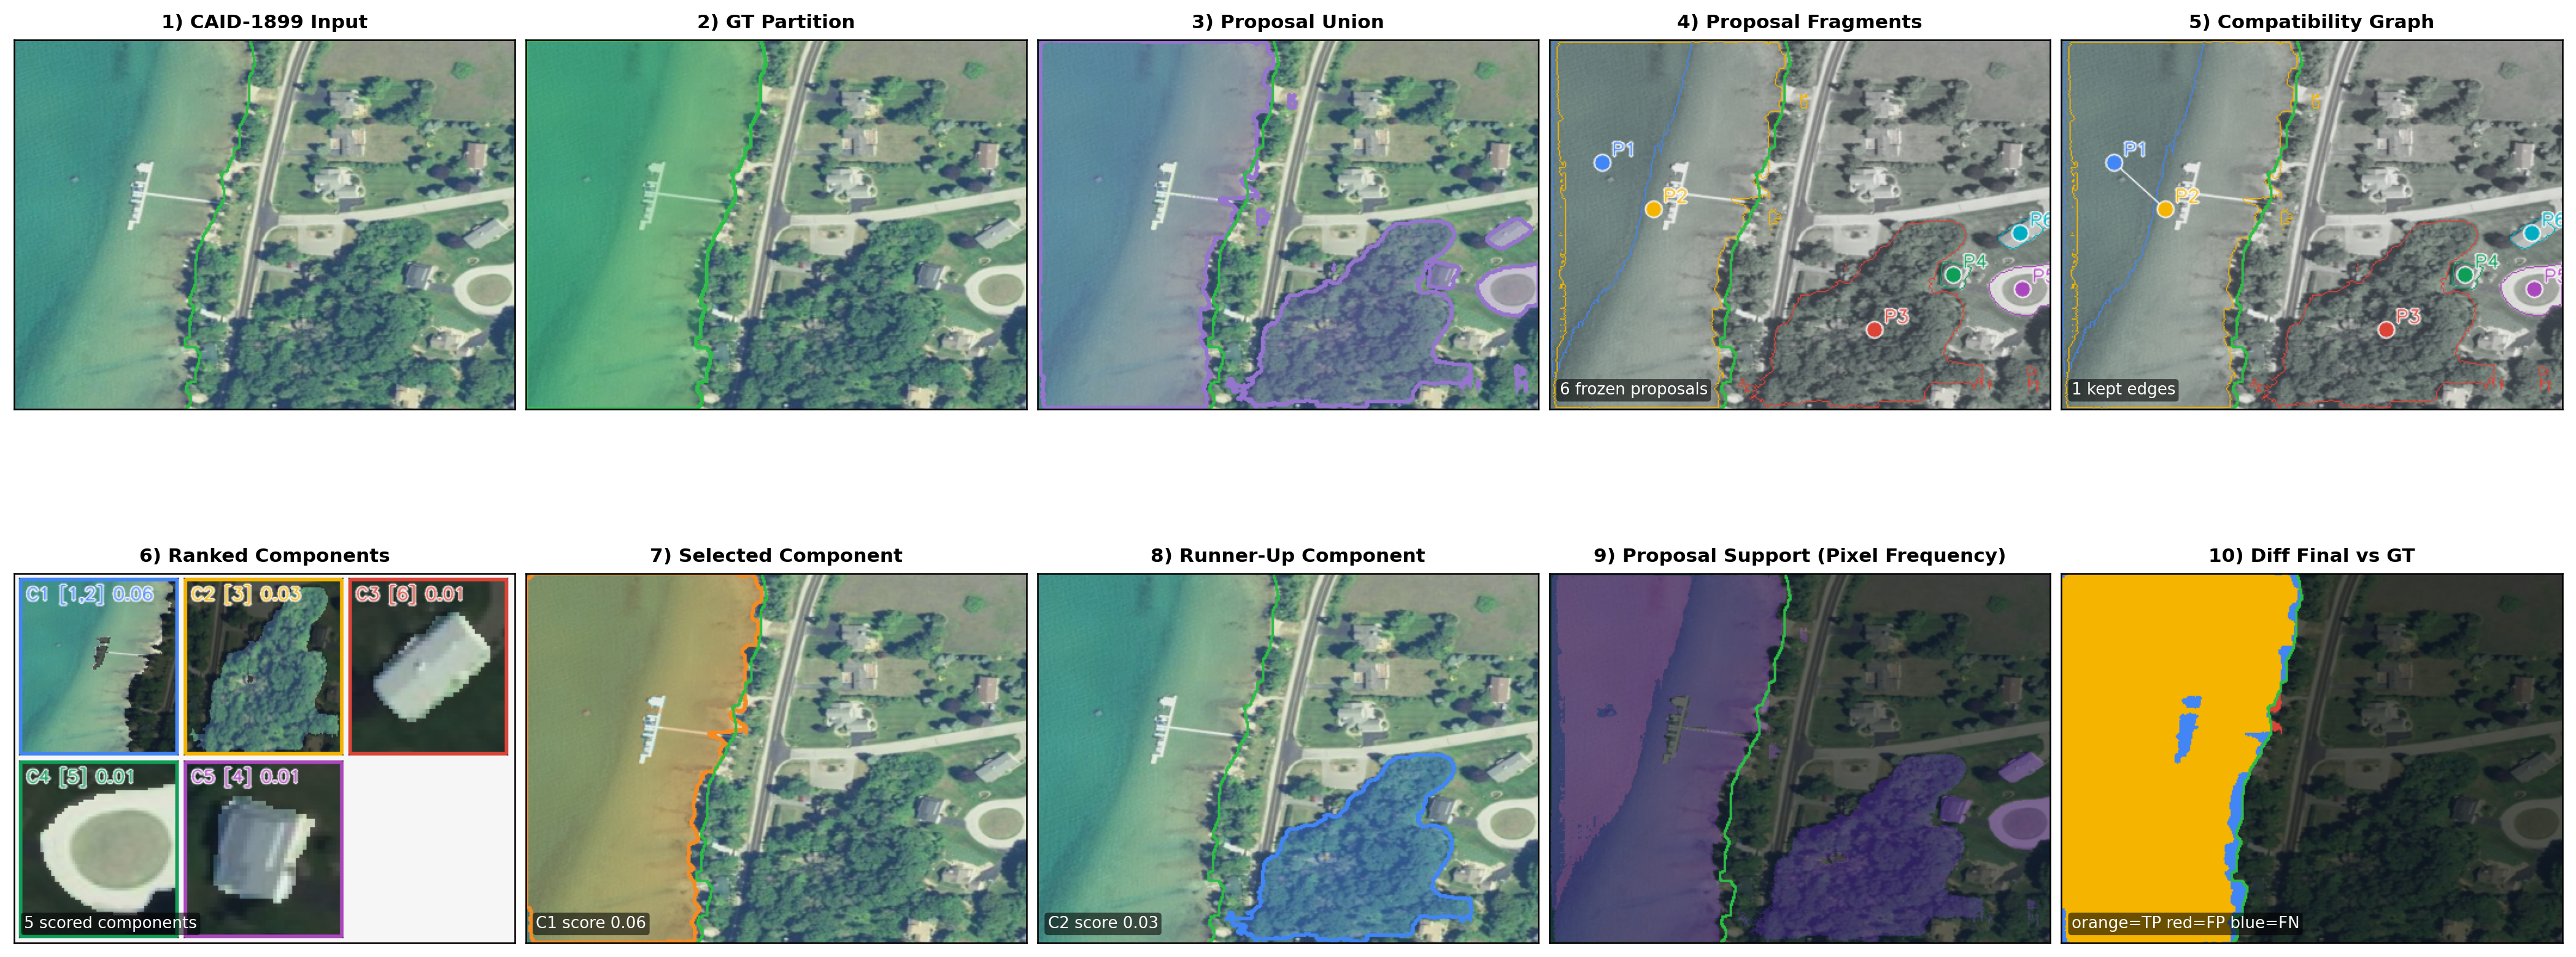
\includegraphics[width=0.98\textwidth]{figures/fig_caid_audit.png}
    \caption{CAID breadth-check example. The same frozen-bank consolidation logic remains useful under shoreline structure, but this route is not central to the paper's texture claim and is reported only as an appendix-side generalization check.}
    \label{fig:caid_app}
\end{figure*}

\begin{table*}[t]
\centering
\scriptsize
\begin{tabularx}{\textwidth}{@{}Xlc@{}}
\toprule
Method & Subset / coverage & Invariant mIoU / ARI \\
\midrule
TextureSAM public checkpoint rerun & all-3104, 3063/3104 & 0.6691 / 0.5080 \\
Proposal route Stage-A & all-3104, 3104/3104 & 0.6677 / 0.5745 \\
TextureSAM public checkpoint rerun & common-3063 & 0.6780 / 0.5148 \\
Proposal route Stage-A & common-3063 & 0.6677 / 0.5745 \\
\bottomrule
\end{tabularx}
\caption{CAID appendix real-world complement under the partition-invariant evaluator. CAID is retained separately because its exact shoreline masks and large contiguous land/water partitions are useful but narrower than the paper's central natural/synthetic texture settings.}
\label{tab:caid_secondary}
\end{table*}

